%%%%%%%%%%%%%%%%%%%%%%%%%%%%%%%%%%%%%%%%%%%%%%%%%%%%
%%%             Metadata                         %%%
%%%%%%%%%%%%%%%%%%%%%%%%%%%%%%%%%%%%%%%%%%%%%%%%%%%%      

\title{Grundkurs Linguistik}

\subtitle{Syntax II: Einführung \& Terminologie}

\author[aMyP]{
	{\small Antonio Machicao y Priemer}
%	\\
%	{\footnotesize \url{http://www.linguistik.hu-berlin.de/staff/amyp}\\
%	\href{mailto:mapriema@hu-berlin.de}{mapriema@hu-berlin.de}}
}

\institute{Institut für deutsche Sprache und Linguistik}

%%%%%%%%%%%%%%%%%%%%%%%%%      
\date{22.\ Juni 2016}
%\publishers{\textbf{6. linguistischer Methodenworkshop \\ Humboldt-Universität zu Berlin}}

%\hyphenation{nobreak}


%%%%%%%%%%%%%%%%%%%%%%%%%%%%%%%%%%%%%%%%%%%%%%%%%%%%
%%%             Preamble's End                   %%%
%%%%%%%%%%%%%%%%%%%%%%%%%%%%%%%%%%%%%%%%%%%%%%%%%%%%      


%%%%%%%%%%%%%%%%%%%%%%%%%      
\huberlintitlepage
\iftoggle{toc}{
\frame{
\begin{multicols}{2}
	\frametitle{Inhaltsverzeichnis}\tableofcontents
	%[pausesections]
\end{multicols}
	}
	}


%%%%%%%%%%%%%%%%%%%%%%%%%%%%%%%%%%
%%%%%%%%%%%%%%%%%%%%%%%%%%%%%%%%%%
%%%%%LITERATURE:

\nocite{Brandt&Co06a} \nocite{Glueck05a} \nocite{Grewendorf&Co91a} \nocite{Luedeling2009a} \nocite{Meibauer&Co07a} \nocite{MuellerS13f} \nocite{MuellerS15b}\nocite{Repp&Co15a} \nocite{Stechow&Sternefeld88a}


%%%%%%%%%%%%%%%%%%%%%%%%%%%%%%%%%%
%%%%%%%%%%%%%%%%%%%%%%%%%%%%%%%%%%
\section{Was bisher geschah \dots }
%\frame{
%\frametitle{~}
%	\tableofcontents[currentsection]
%}


%%%%%%%%%%%%%%%%%%%%%%%%%%%%%%%%%%
\begin{frame}
\frametitle{Was bisher geschah \dots }

\begin{itemize}
	\item Sie wissen:
	\begin{itemize}
		\item womit sich Syntax befasst,
		\item wie man Syntax definieren kann,
		\item dass man auch \textbf{Konstituenten} und \textbf{Kategorien} beziehen muss,
		\item dass \textbf{Linearität} $\neq$ \textbf{Struktur},
		\item was der Unterschied zwischen \textbf{Grammatikalität} und \textbf{Akzeptabilität} ist,
		\item was der Unterschied zwischen \textbf{deskriptiv} und \textbf{präskriptiv} ist.
	\end{itemize}
\end{itemize}

\end{frame}


%%%%%%%%%%%%%%%%%%%%%%%%%%%%%%%%%%
%%%%%%%%%%%%%%%%%%%%%%%%%%%%%%%%%%
\section{Generative Grammatik}
%\frame{
%\frametitle{~}
%	\tableofcontents[currentsection]
%}


%%%%%%%%%%%%%%%%%%%%%%%%%%%%%%%%%%
\begin{frame}
\frametitle{Generative Grammatik}

\begin{itemize}
	\item Wie gelangen wir zu den deskriptiven Regeln, um die (Un-)Grammatikalität innerhalb eines Regelapparats zu modellieren?

\pause

	\item[]
	\item  \textbf{Sprachliche Intuition} \ras Sprecher haben ein Gefühl dafür, was sie in ihrer Muttersprache sagen \gqq{können} und was \gqq{nicht}. Durch \textbf{Introspektion} (Selbstbefragung) gelangen sie zu diesem Wissen. Dadurch befragen sie ihre sog. muttersprachliche Kompetenz.

\end{itemize}

\end{frame}


%%%%%%%%%%%%%%%%%%%%%%%%%%%%%%%%%%
\begin{frame}
\frametitle{Generative Grammatik}

\begin{itemize}

	\item Sprachliche Intuition \ras wesentlich in den sog. generativen Syntaxtheorien seit \citet{Chomsky57a}

\begin{figure}
\centering
	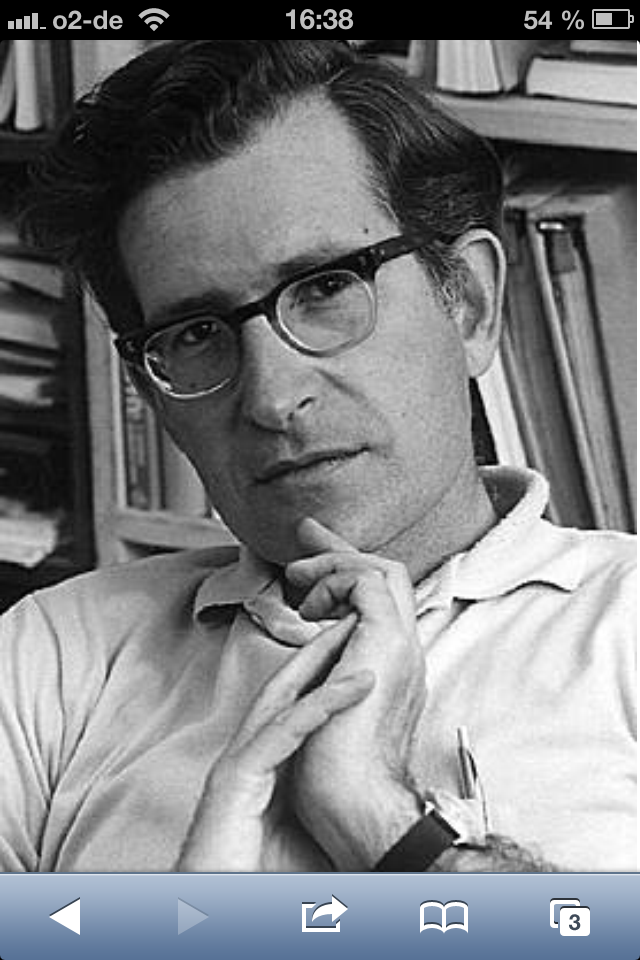
\includegraphics[scale=.17]{material/03chomsky}
\end{figure}

	
\end{itemize}

\end{frame}


%%%%%%%%%%%%%%%%%%%%%%%%%%%%%%%%%%
\begin{frame}
\frametitle{Generative Grammatik}

\begin{itemize}

	\item Sprachliche Intuition \ras wesentlich in den sog. generativen Syntaxtheorien seit \citet{Chomsky57a}

\begin{figure}
\centering
	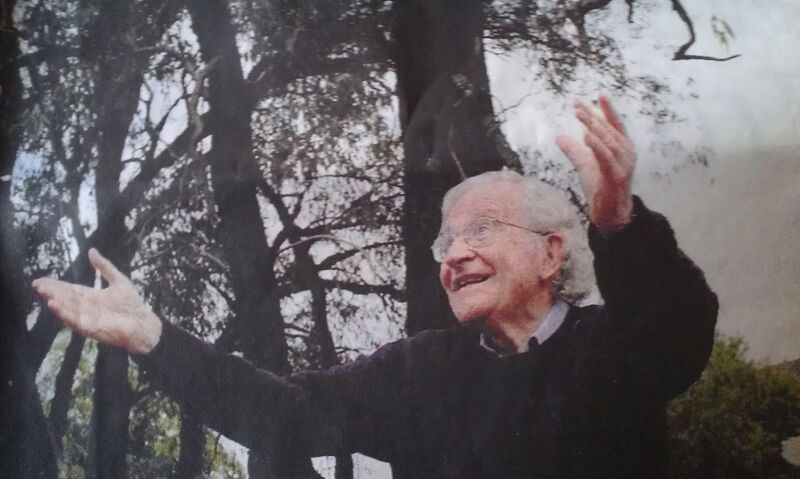
\includegraphics[scale=.3]{material/04chomsky}
\end{figure}

	
\end{itemize}

\end{frame}


%%%%%%%%%%%%%%%%%%%%%%%%%%%%%%%%%%
\begin{frame}
\frametitle{Generative Grammatik}

\begin{itemize}
	\item Was ist diese Generative Grammatik?
	\item[]
	\item Seit \citet{Chomsky57a} und \citet{Chomsky65a}
	\item[]
	\item \textbf{Dynamische Theorie} (vgl. Statische Theorie \ras \zB Strukturalismus)
	\begin{itemize}
		\item Grammatik als dynamisches System \ras Regelsystem, das wohlgeformte Strukturen \emph{erzeugt}
		\item[]
		\item Strukturalistisches Konzept \gqq{Langue} setzt ein statisches Zeichensystem voraus. 
	\end{itemize}

\end{itemize}

\end{frame}


%%%%%%%%%%%%%%%%%%%%%%%%%%%%%%%%%%
\begin{frame}
\frametitle{Generative Grammatik}

\begin{itemize}
	\item Klare Definition des Untersuchungsgegenstandes \gqq{Sprache}:
	\begin{itemize}
		\item Keine Beschreibung mehr von \gqq{sprachlichen} Phänomenen, ohne davor den Begriff \gqq{Sprache} zu definieren / einzuschränken.
		\item[]
		\item \textbf{I-Language} \ras intrinsische Kompetenz des idealen Sprecher-Hörers (Trennung zw. Kompetenz und Performanz)
	\end{itemize}
	\item[]
	\item Linguistik als Wissenschaft \ras durch Formalisierung
	\item[]
	\item \textbf{Rationalistische} Vorgehensweise (Cartesianische Linguistik)
	\begin{itemize}
		\item Bruch mit behaviouristischer Vorgehensweise (Empirismus)
		\item Rationalistische Sichtweise des Spracherwerbs
		\item Universalgrammatik \ras genetisch verankerte Grundlage der menschlichen Sprachfähigkeit
	\end{itemize}
\end{itemize}

\end{frame}


%%%%%%%%%%%%%%%%%%%%%%%%%%%%%%%%%%
\begin{frame}
\frametitle{Generative Grammatik}

\begin{itemize}
	\item Verwandtschaft zwischen Sätzen erkennen, beschreiben und erklären (Erklärungsadäquatheit) \ras Transformationen
	
	\eal 
	\ex Man kauft Bier.
	\ex Bier wird gekauft.
	\zl
	
	\item[]	
	\item Beschreibung von sprachlichen Phänomenen ist nicht das primäre Ziel.
\end{itemize}

\end{frame}


%%%%%%%%%%%%%%%%%%%%%%%%%%%%%%%%%%
\begin{frame}
\frametitle{Generative Grammatik}

\begin{block}{Ziel generativer Theorien}
Durch eine \textbf{deskriptive} Vorgehensweise wird ein Regelapparat erstellt, um \textbf{lineare} und \textbf{hierarchische} Gesetzmäßigkeiten des Satzbaus zu \textbf{beschreiben}. Daraus wird versucht, allgemeine (\textbf{universelle}) Gesetzmäßigkeiten der menschlichen Sprachfähigkeit abzuleiten, um somit die menschliche (Sprach)\textbf{Kompetenz zu erklären}.
\end{block}

\end{frame}


%%%%%%%%%%%%%%%%%%%%%%%%%%%%%%%%%%
%%%%%%%%%%%%%%%%%%%%%%%%%%%%%%%%%%
\subsection{Kompetenz vs. Performanz}
%\frame{
%\frametitle{~}
%	\tableofcontents[currentsection]
%}


%%%%%%%%%%%%%%%%%%%%%%%%%%%%%%%%%%
\begin{frame}
\frametitle{Kompetenz \vs Performanz}

\begin{block}{Kompetenz}
Sprachfähigkeit. Ein mental (\gqq{im Geist}) verankertes \textbf{unbewusstes Wissenssystem von Regeln}, das der Produktion und Rezeption unendlich vieler Sätzen zugrunde liegt (auch: I-Sprache für internalisierte Sprache).
\end{block}	


\end{frame}


%%%%%%%%%%%%%%%%%%%%%%%%%%%%%%%%%%
\begin{frame}
\frametitle{Kompetenz \vs Performanz {\footnotesize \citep[vgl.][16ff.]{Brandt&Co06a}}}

\begin{itemize}
	\item Die Kompetenz äußert sich in der Fähigkeit:

	\begin{itemize}
		\item[]
		\item Sätze einer Sprache als \textbf{grammatisch oder ungrammatisch} zu beurteilen,

\pause		
\only<2>{
		\ea \alert{Peter$_i$} rasiert \{\alert{*ihn$_i$/sich$_i$}\}.
		\z
		
		\ea \alert{Peter$_i$} freut sich, dass man \{\alert{ihn$_i$/*sich$_i$}\} gelobt hat.
		\z
		}

\pause	
		\item[]	
		\item \textbf{strukturell verwandte} Sätze zu erkennen,
\pause
\only<4>{
		\ea Man kauft ein Haus.
		\z
		
		\ea Ein Haus wird gekauft.
		\z
		}

\pause	
		\item[]	 
		\item \textbf{strukturelle und lexikalische Ambiguitäten} zu erkennen,
\pause
\only<6>{
		\ea Peter traf \alert{die Frau mit dem roten Schuh}.
		\z
		
		\ea Peter liebt die \alert{Schule}.
		\z
		}

\pause	
		\item[]	 
		\item \textbf{syntaktisch wohlgeformte Äußerungen} zu erkennen, auch wenn der Inhalt unsinnig ist.
\pause
\only<8>{
		\ea[]{Viele hartnäckig verheiratete Jungessellen stehen intensiv.}
		\z
		
		\ea[*]{Hartnäckig intensiv Jungessellen stehen verheiratete viele.}
		\z
		}
		
	\end{itemize}
\end{itemize}
\end{frame}


%%%%%%%%%%%%%%%%%%%%%%%%%%%%%%%%%%
\begin{frame}
\frametitle{Kompetenz \vs Performanz}

\begin{figure}
\centering
	
\includegraphics[scale=.5]{material/08ambiguity}
	\caption{Ambiguität}
\end{figure}

\end{frame}


%%%%%%%%%%%%%%%%%%%%%%%%%%%%%%%%%%
\begin{frame}
\frametitle{Kompetenz vs. Performanz}

\begin{block}{Performanz}
Sprachverwendung. Anwendung der Sprachfähigkeit in einer konkreten Sprechsituation.
\end{block}

\end{frame}


%%%%%%%%%%%%%%%%%%%%%%%%%%%%%%%%%%
\begin{frame}
\frametitle{Kompetenz vs. Performanz}

\begin{itemize}
	\item Die Performanz weicht oft von der Kompetenz ab: 
	\begin{itemize}
		\item[]
		\item Sprecher versprechen sich, 
		
\pause		
%\only<2>{
		\ea Ich hätte gerne einen Kilchmaffee\dots\ Ähm! Ich meine einen MILCHKaffee.
		\z
%		}

\pause
		\item[]		
		\item brechen mitten im Satz ab,
\pause		
%\only<4>{
		\ea Ich wollte ja noch \dots\ Ach, nichts!
		\z
%		}
		 
		\item[] 
		\item wiederholen Wörter.
\pause		
%\only<6>{
		\ea Ich hab ich hab ich hab gestern noch den Film geguckt.
		\z
%		}
		
		\item[]
		\item[]	Aber niemand würde daraus schließen, dass sie ihre Muttersprache nicht beherrschen.
	\end{itemize}

\end{itemize}

\end{frame}


%%%%%%%%%%%%%%%%%%%%%%%%%%%%%%%%%%
\begin{frame}
\frametitle{Kompetenz vs. Performanz}

\begin{itemize}

	\item Die Unterscheidung grammatisch-ungrammatisch spiegelt die Kompetenz des \textbf{idealen Sprecher-Hörers} wider.
\end{itemize}

\begin{block}{Idealer Sprecher-Hörer}
Theoretisches (und nicht unumstrittenes) Konstrukt innerhalb der Generativen Grammatik, um die Sprachdaten, mit denen gearbeitet wird, von \gqq{Performanzeffekten zu bereinigen}. Notwendig für eine Abgrenzung des Untersuchungsgegenstandes der GG.
\end{block}

\begin{itemize}
	\item Die verschiedenen Akzeptabilitätsgrade haben häufig mit Performanzeffekten zu tun.
	\item[]
	\item Die Kompetenz-Performanz-Dichotomie wird in einigen (gebrauchsbasierten) Frameworks (\zB Construction Grammar) abgelehnt \citep[vgl.][]{MuellerS15b, Nolda&Co14a}. 
\end{itemize}

\end{frame}


%%%%%%%%%%%%%%%%%%%%%%%%%%%%%%%%%%
%%%%%%%%%%%%%%%%%%%%%%%%%%%%%%%%%%
\subsection{Universalgrammatik}
%\frame{
%\frametitle{~}
%	\tableofcontents[currentsection]
%}


%%%%%%%%%%%%%%%%%%%%%%%%%%%%%%%%%%%
\begin{frame}
\frametitle{Universalgrammatik (UG)}

\begin{itemize}

	\item Die (menschliche) natürliche Sprache unterscheidet sich von der Sprache anderer Tiere in vielerlei Hinsicht. \citep[vgl. \zB ][]{Hockett60a, Pinker95a}\\
	(Gegenargumente und Diskussion: \citet{Evans&Levinson09a, MuellerS15b})
	\item[]
	\item Welche sind die Merkmale, die eine \textbf{natürliche Sprache} von anderen Sprachen unterscheiden? 
	\begin{itemize}
		\item Produktivität, Bidirektionalität, Arbitrarität, Diskretheit, Rekursivität, \dots \citep[vgl.][]{Luedeling2009a}
	\end{itemize}
	\item[]
	\item Andere Primaten können bspw. lexikalische Einträge erwerben (25--125 lexikalische Einträge), aber keine abstrakten Regeln!
\end{itemize}

\end{frame}


%%%%%%%%%%%%%%%%%%%%%%%%%%%%%%%%%%
\begin{frame}
\frametitle{Universalgrammatik}

\begin{figure}
\centering
	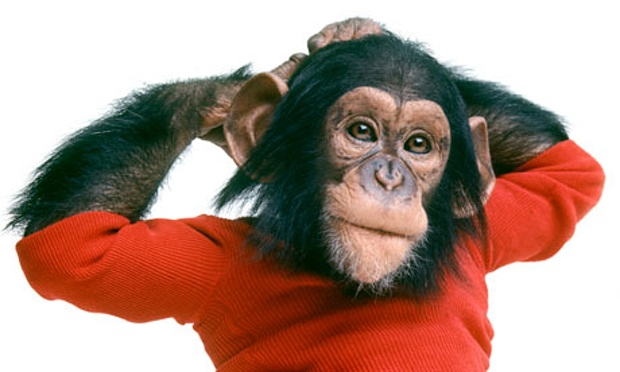
\includegraphics[scale=.3]{material/06nimchimpsky}
	\caption{Nim Chimpsky}
\end{figure}

\begin{itemize}
	\item Siehe \textbf{Nim Chimpsky}: \url{https://en.wikipedia.org/wiki/Nim_Chimpsky}
	\ea Give orange me give eat orange me eat orange give me eat orange give me you. \hfill (Nim Chimpsky)
	\z

\end{itemize}

\end{frame}


%%%%%%%%%%%%%%%%%%%%%%%%%%%%%%%%%%
\begin{frame}
\frametitle{Universalgrammatik}

\begin{itemize}
	\item \textbf{Erwerbbarkeit} von Regeln 
	\begin{itemize}
		\item Dem Kind muss es möglich sein, \textbf{abstrakte Regeln} zu erwerben.
		\item[]
		\item Mit welcher Sprachausstattung kommt das Kind zur Welt? \ras UG
		\item[]
		\item Wie müssen Regeln aussehen, damit sie mit dieser angeborenen Sprachausstattung (UG) erworben werden können?
		\item[]
		\item \textbf{Mentalistischer Nativismus} in der \textbf{rationalistischen} Tradition von Descartes und Humboldt (vs. empiristische Tradition) \ras Große Bereiche kognitiver Strukturen sind \textbf{genetisch} vorgegeben sind (vgl. Biolinguistik \ras FOXP2) \citep[vgl.][]{Hornstein05a}
		\item[]
		\item Angeborene Sprachausstattung \ras Set von Prinzipien \ras UG		
	\end{itemize}
\end{itemize}

\end{frame}


%%%%%%%%%%%%%%%%%%%%%%%%%%%%%%%%%%
\begin{frame}
\frametitle{Universalgrammatik}

\begin{itemize}
	\item \textbf{Argument vom defizienten Input} (Poverty-of-the-Stimulus Argument) beim Spracherwerb:
	
	\begin{itemize}
		\item Das Kind bekommt nur sog. positive Evidenz beim Erlernen \ras aber nur Performanzdaten!
		\item[]
		\item Vorkommen von Fehlern
		\item[]
		\item Korrekturen \ras nicht bei jeder falschen Äußerung
		\item[]
		\item Unterschiedliche Leute korrigieren unterschiedlich
		\item[]
		\item Trotzdem lernen alle Kinder ihre Muttersprache auf dieselbe Art und Weise in ungefähr der gleichen Zeit \citep[vgl.][18ff.]{Philippi&Tewes10a}
		\item[]
		\item Das deutet daraufhin, dass das Kind schon mit einer gewissen Sprachkompetenz (Set sprachlicher Prinzipien oder UG) geboren wird.

	\end{itemize}

\end{itemize}

\end{frame}


%%%%%%%%%%%%%%%%%%%%%%%%%%%%%%%%%%
\begin{frame}
\frametitle{Universalgrammatik}

\begin{itemize}
	\item \textbf{Argument vom defizienten Input} (Poverty-of-the-Stimulus Argument) beim Spracherwerb (vgl. \citet{Lasnik&Co02a} vs. \citet{Pullum&Scholz02a}):
	\item[]
	\item Prinzip der \textbf{Strukturabhängigkeit:}
	\eal 
	\ex[]{Der Hund \alert{ist} hungrig.}
\pause
	\ex[]{\alert{Ist} der Hund hungrig?}
\pause
	\ex[]{Der Hund, der an der Ecke \alert{ist}, \alert{ist} hungrig.}
\pause	
	\ex[*]{\alert{Ist}$_{i}$ der Hund, der an der Ecke \alert{t}$_{i}$, \alert{ist} hungrig?}
\pause
	\ex[]{\alert{Ist}$_{i}$ der Hund, der an der Ecke \alert{ist}, \alert{t}$_{i}$ hungrig?}
	\zl

\pause	

	\eal 
	\ex \alert{Er}$_{\neq 1, =2}$ hat gesagt, dass \alert{Peter}$_1$ Maria mag.
\pause	
	\ex \alert{Peter}$_1$ hat gesagt, dass \alert{er}$_{=1, =2}$ Maria mag.
\pause	
	\ex Dass \alert{er}$_{=1, =2}$ Maria mag, hat \alert{Peter}$_1$ gesagt.
	\zl
	
	
\end{itemize}

\end{frame}


%%%%%%%%%%%%%%%%%%%%%%%%%%%%%%%%%%
\begin{frame}
\frametitle{Universalgrammatik}

\begin{itemize}
	\item \textbf{Kreativitätsargument}
	\item[]
	\item Mit einer \textbf{begrenzten Anzahl an Phonemen}, kann man eine \textbf{begrenzte Anzahl an Wörtern} generieren, mit denen man aber \textbf{eine unendliche Menge an Sätzen} produzieren und verstehen kann.

\pause	
	\ea Karl-Heinrich hat trotz seiner Seekrankheit genügende Argumente, um für die bessere Behandlung der Flüchtlinge in seinem Bezirk zu demonstrieren.
	\z

\end{itemize}

\end{frame}


%%%%%%%%%%%%%%%%%%%%%%%%%%%%%%%%%%
\begin{frame}
\frametitle{Universalgrammatik}

\begin{itemize}
	\item \textbf{Argument der Übergeneralisierung}
	\item[]
	\item Fehler von Kindern weisen auf die Anwendung von Regeln hin (Übergeneralisierung).

\pause	
	\eal 
	\ex geben
	\ex gegebt
	\zl
	
	\eal 
	\ex A: Schläfst du?
	\ex B: Ja, ich schläfe.
	\zl
	
	\eal 
	\ex das Schaf
	\ex die Schäfe (vgl. der Ball -- die Bälle).
	\zl

\end{itemize}

\end{frame}


%%%%%%%%%%%%%%%%%%%%%%%%%%%%%%%%%%
\begin{frame}
\frametitle{Universalgrammatik}

\begin{itemize}
	\item Unterschiedliche Sprachen auf der Welt aber nur \textbf{eine UG}? \ras \textbf{Prinzipien vs. Parameter}

	\begin{block}{Prinzipien}
	Universelle Regeln, nach denen mögliche Sprachen gebildet werden und unmögliche ausgeschlossen werden. 
	\end{block}
	
	\item \textbf{Kopfprinzip:} Jede Phrase hat einen und nur einen Kopf.

\pause
	\eal 
	\ex[]{[Kekse$_ {N}$ backen$_ {V}$ $_ {VP}$]}
	\ex[*]{[Kekse$_ {N}$ backen$_ {V}$ $_ {NP}$]}
	\ex[*]{[Kekse$_ {N}$ backen$_ {V}$ $_ {VP \& NP}$]}
	\zl
	
\end{itemize}

\end{frame}


%%%%%%%%%%%%%%%%%%%%%%%%%%%%%%%%%%
\begin{frame}
\frametitle{Universalgrammatik}

\begin{itemize}

	\begin{block}{Parameter}
	Einzelsprachlich spezifische Regeln, die Möglichkeiten darstellen, die universalgrammatischen Prinzipien auszubuchstabieren.
	\end{block}
	
	\item Durch den Input der Zielsprache werden sog. \textbf{Parameter} gesetzt
	\item[]
	\item \textbf{Kopfparameter:} Position des Kopfes einer Phrase (vgl. Prinzip der Rechtsköpfigkeit in der Morphologie)
	
	\eal
	\ex Dt.: das grüne \alert{Haus}
	\ex
	\gll Sp.: la \alert{casa} verde\\
		{} das Haus grün\\
	\zl
	
	\item Ein Adjektiv kann in einer Nominalphrase in Abhängigkeit von der jeweiligen Sprache links oder rechts vom Nomen stehen.


\end{itemize}

\end{frame}


%%%%%%%%%%%%%%%%%%%%%%%%%%%%%%%%%%
\begin{frame}
\frametitle{Universalgrammatik}

\begin{itemize}
	\item Inventar an Prinzipien und Parametern ist beschränkt (aus Ökonomiegründen)
	\item[]
	\item Prinzipien und Parameter sind Teil unserer grammatischen Kompetenz.
	\item[]
	\item \textbf{Kerngrammatik} = UG + sprachspezifische Parameter
	\item \textbf{Einzelgrammatik} = Kerngrammatik + Peripherie
	\item[]
	\item Peripherie: Entlehnungen, historische Residuen, Erfindungen, Ausnahmen \citep[vgl.][]{Nolda&Co14a}
	\eal
	\ex sterben -- starb -- gestorben
	\ex Forelle blau
	\ex sitt (\url{https://de.wikipedia.org/wiki/Sitt})
	\ex In den Müll damit!
	\zl
	
\end{itemize}

\end{frame}


%%%%%%%%%%%%%%%%%%%%%%%%%%%%%%%%%%
\begin{frame}
\frametitle{Universalgrammatik}

\begin{block}{Ziel generativer Theorien}
In einer \textbf{deskriptiven} Vorgehensweise werden Phänomene adäquat \textbf{beobachtet} und deren \textbf{linearen} und \textbf{hierarchischen} Regelmäßigkeiten adäquat \textbf{beschrieben}, dabei werden die \textbf{Performanz}phänomene und die Elemente der \textbf{Peripherie} aus der Untersuchung ausgeschlossen. Aus den Phänomenen der \textbf{Kerngrammatik} wird versucht, allgemeine (\textbf{universelle}) Gesetzmäßigkeiten der menschlichen Sprachfähigkeit abzuleiten (\textbf{Prinzipien und Parameter \ras UG}), um somit die menschliche (Sprach)\textbf{Kompetenz} zu \textbf{erklären}.
\end{block}

Schlagen Sie \gqq{Adäquatheit} in \citet{Glueck05a} nach!

\end{frame}


%%%%%%%%%%%%%%%%%%%%%%%%%%%%%%%%%%
%%%%%%%%%%%%%%%%%%%%%%%%%%%%%%%%%%
\section{Wortarten}
%\frame{
%\frametitle{~}
%	\tableofcontents[currentsection]
%}


%%%%%%%%%%%%%%%%%%%%%%%%%%%%%%%%%%
\begin{frame}
\frametitle{Wortarten}

\begin{itemize}
	\item \textbf{Klassifikation} des Wortschatzes unter grammatischen Gesichtspunkten 
	\item[]

\pause	

	\ea Raustorf ergt schrubbenes Klot.
	\z

\pause

	\ea Raustorf$_N$ ergt$_V$ schrubbenes$_A$ Klot$_N$.
	\z
	
\pause
	\item \textbf{Semantische Klassifikation}:
	\begin{itemize}
		\item Elemente, die auf \textbf{Entitäten} referieren \ras Substantive
		\item Elemente, die auf \textbf{Eigenschaften} referieren \ras Adjektive
		\item Elemente, die eine \textbf{Handlung} ausdrücken \ras Verben

	\end{itemize}

\pause
	\item[]
	\item Kriterien für die Klassifikation \ras \textbf{morphologisch, syntaktisch, semantisch, (pragmatisch)}
	
\end{itemize}

\end{frame}


%%%%%%%%%%%%%%%%%%%%%%%%%%%%%%%%%%
\begin{frame}
\frametitle{Wortarten}

\begin{itemize}
	\item Klassifikation von Wörtern in Oberkategorien \ras bereits in der klassischen griechischen Grammatik
	\item[]
	\item Wortartenklassifikation von Dionysius Thrax (200--100 v. Chr.):
\pause
	\begin{itemize}
		\item Nomen,
		\item Verb, 
		\item Pronomen,
		\item Präposition,
		\item Adverb,
		\item Konjunktion,
		\item Partizip,
		\item Artikel
	\end{itemize}
\pause
	\begin{itemize}
		\item Adjektiv,
		\item Partikeln,
		\item Interjektionen \dots
	\end{itemize}
\end{itemize}

\end{frame}


%%%%%%%%%%%%%%%%%%%%%%%%%%%%%%%%%%
\begin{frame}
\frametitle{Wortarten}

\begin{itemize}
	\item \textbf{Positionsbasierte Definition:}\\
	Position des Wortes im Satz in Relation zu anderen Wörtern
	\begin{itemize}
		\item Adjektive stehen zwischen einem Artikel und dem Nomen, auf das sie sich beziehen.
		\item Verben besetzen \idR die \gqq{zweite Position} in einem Aussagesatz oder die letzte Position in einem Nebensatz
		\item Problem: attributive \vs prädikative Adjektive.
	\end{itemize}

	\item[]
	\item \textbf{Merkmalbasierte Definition:}\\
	nach bestimmten \textbf{Flexionsmerkmalen} (Kasus und Numerus bei Nomina), nach \textbf{syntaktischer Funktion} (\idR können Nomina Subjekt oder Objekt eines Satzes sein), nach \textbf{semantischen Merkmalen} (Nomina sind eher Entitäten mit Referenz)


\end{itemize}

\end{frame}


%%%%%%%%%%%%%%%%%%%%%%%%%%%%%%%%%%
\begin{frame}
\frametitle{Wortarten}

\begin{figure}
\centering
	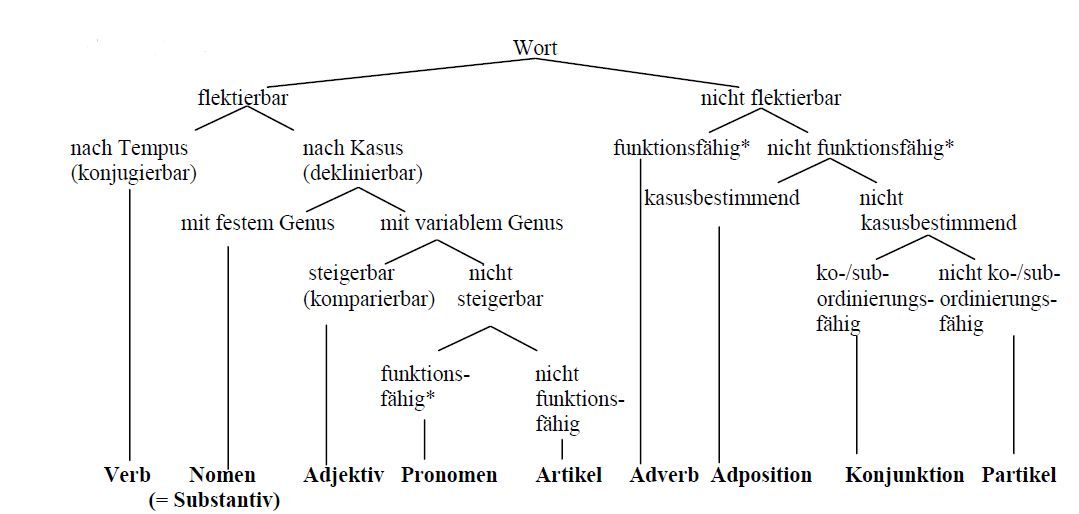
\includegraphics[scale=.4]{material/07wortartenklassifikation}
	\caption{Wortartenklassifikation \citep{Repp&Co15a}}
\end{figure}

\end{frame}


%%%%%%%%%%%%%%%%%%%%%%%%%%%%%%%%%%
\begin{frame}
\frametitle{Wortarten}

\begin{itemize}
	\item \textbf{Schwierigkeiten} mit prototypischen Eigenschaften:

	\eal 
	\ex mithilfe 
	\ex mit Hilfe
	\zl
	
\pause 
Präposition oder Präposition + Nomen (+ Nomen im Genitiv?)
\pause

	\ea bausparen 
	\z

\pause	
	nicht V2-fähig wie die \gqq{gewöhnlichen} Verben
\pause

	\ea Das \textbf{Schlafen}
	\z

\pause
Verb oder Nomen?
\pause

	\eal
	\ex Er \textbf{kauft} Brot. 
	\ex Er hat das Brot \textbf{gekauft}.
\pause
	\ex Das \textbf{gekaufte} Brot
	\zl
	
\pause
Verb oder Adjektiv?

\end{itemize}

\end{frame}


%%%%%%%%%%%%%%%%%%%%%%%%%%%%%%%%%%
\begin{frame}
\frametitle{Wortarten}

\begin{itemize}

	\item In unserem Kurs:

\end{itemize}

\begin{table}
\centering
\scalebox{0.9}{
\begin{tabular}{lll}
\textbf{Wortart} & \textbf{Abk.} & \textbf{Beispiel} \\ 
\hline
Nomen (Substantiv) & N & Tisch, Liebe, Maria \\ 
\hline
Determinierer (Artikel, Quantor, Pronomen) & D & der, dem, alle, ein, ich \\ 
\hline
Adjektiv & A & schön, syntaktisch \\ 
\hline
Adverb & Adv & heute, hier \\ 
\hline
Verb & V & rennen, malen \\ 
\hline
Adposition (Prä- \& Postposition) & P & vor, in, wegen, entlang \\ 
\hline
Komplementierer (Subjunktion) & C & ob, dass, weil \\ 
\hline
Konjunktion & K & und, aber, sondern \\ 
\hline
Partikel & Part & ja, wohl, leider \\ 
\hline
\end{tabular} 
}

\end{table}

\end{frame}


%%%%%%%%%%%%%%%%%%%%%%%%%%%%%%%%%%
%%%%%%%%%%%%%%%%%%%%%%%%%%%%%%%%%%
\section{Konstituenten}
%\frame{
%\frametitle{~}
%	\tableofcontents[currentsection]
%}


%%%%%%%%%%%%%%%%%%%%%%%%%%%%%%%%%%
\begin{frame}
\frametitle{Konstituenten}

\begin{itemize}
	\item Nicht nur Wörter, sondern auch größere Einheiten spielen in der Syntax eines Satzes eine wichtige Rolle.
	\item[]
	\item Pausen beim Vorlesen:
	\ea Eine 16 Jahre alte Französin starb nach dem Verzehr eines Döners an Lebensmittelvergiftung.\jambox{(Quelle: \url{www.frauenzimmer.de})}
	\z
	
\pause	
	\item Verschiebungen in einem Satz:
	\eal 
	\ex[]{Eine 16 Jahre alte Französin starb \alert{[nach dem Verzehr]} eines Döners an Lebensmittelvergiftung.}
	\ex[]{\alert{[Nach dem Verzehr eines Döners]} starb eine 16 Jahre alte Französin an Lebensmittelvergiftung.}
	\ex[*]{\alert{[Nach dem Verzehr]} starb eine 16 Jahre alte Französin \alert{[eines Döners]} an Lebensmittelvergiftung.}
	\zl


\end{itemize}

\end{frame}


%%%%%%%%%%%%%%%%%%%%%%%%%%%%%%%%%%
\begin{frame}
\frametitle{Konstituenten}

\begin{itemize}
	\item Wörter bilden (\textbf{konstituieren}) mit anderen Wörtern Konstituenten, die dann gemeinsam größere Konstituenten bilden (s. Morphologie!)
	
	\eal
	\ex [eines] + [Döners] = [eines Döners]
\pause	
	\ex [Verzehr] + [eines Döners] = [Verzehr eines Döners]
\pause
	\ex [dem] + [Verzehr eines Döners] = [dem Verzehr eines Döners]
\pause
	\ex [nach] + [dem Verzehr eines Döners] = [nach dem Verzehr eines Döners]
	\zl

\end{itemize}

\end{frame}


%%%%%%%%%%%%%%%%%%%%%%%%%%%%%%%%%%
\begin{frame}
\frametitle{Konstituenten}

\begin{itemize}
	\item Die hierarchische Struktur des Satzes lässt sich in der Gehirnaktivität bei der Verarbeitung erkennen (Siehe \citet{Devitt15a} (Pro Chomsky) vs. \citet{Boutonnet15a} (Gegen Chomsky))	
\end{itemize}

\begin{figure}
\centering
	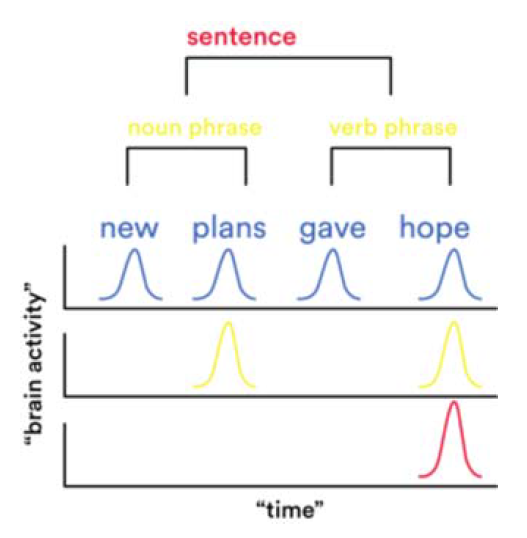
\includegraphics[scale=.35]{material/10gehirnaktivitaet}
	\caption{\citep[Quelle:][]{Boutonnet15a}}
\end{figure}

\end{frame}


%%%%%%%%%%%%%%%%%%%%%%%%%%%%%%%%%%%
\begin{frame}
\frametitle{Konstituenten}

\begin{itemize}
	\item Konstituente: relational zu anderen Konstituenten und zum dem, was sie konstituieren (\ras einfach vs. komplex)
	\item[]
	\item Bei den Konstituenten ist es wichtig herauszufinden, welche sich in Sätzen wie eine \textbf{strukturelle Einheit} verhalten.
	\item[]
	\item In der traditionellen Grammatik \ras Satzgliedern und Satzgliedteilen

\end{itemize}

\end{frame}


%%%%%%%%%%%%%%%%%%%%%%%%%%%%%%%%%%%
\begin{frame}
\frametitle{Konstituenten}

\begin{itemize}

	\item \textbf{Konstituententests} \citep[vgl.][4ff.]{MuellerS13f}
	\begin{itemize}
		\item Ersetzungstest (oder Substitutionstest)
		\item Pronominalisierungstest
		\item Fragetest
		\item Verschiebetest (oder Permutationstest)
		\item Vorfeldtest (oder Voranstellungstest) 
		\item Weglasstest (oder Eliminierungstest)
		\item (Koordinationstest, Parenthesetest, \dots )
	\end{itemize}
	\item[]
	\item (Phrasale) Konstituenten sollten sich in den meisten dieser Tests als Einheit verhalten.

\end{itemize}

\end{frame}


%%%%%%%%%%%%%%%%%%%%%%%%%%%%%%%%%%%
%%%%%%%%%%%%%%%%%%%%%%%%%%%%%%%%%%
\subsection{Eretzungstest}
%\frame{
%\frametitle{~}
%	\tableofcontents[currentsection]
%}

%%%%%%%%%%%%%%%%%%%%%%%%%%%%%%%%%%%
\begin{frame}
\frametitle{Ersetzungstest (Substitutionstest)}

\begin{itemize}
	\item Was sich durch ein anderes Wort (/einer anderen Wortfolge) ersetzen lässt, so dass der Satz grammatisch bleibt, ist (vermutlich) eine (phrasale) Konstituente.

	\eal 
	\ex[]{\alert{[Eine Frau]} starb nach dem Verzehr eines Döners.}
	\ex[]{\alert{[Ein Mann]} starb nach dem Verzehr eines Döners.}
	\ex[*]{\alert{[Ein Mann]} nach dem Verzehr eines Döners.}
	\zl

\pause	
	\eal 
	\ex Die Frau hat versucht, \alert{[den Döner zu genießen]}.
	\ex Die Frau hat versucht, \alert{[uns allen Weihnachtsgeschenke zu geben]}.
	\zl
	
\end{itemize}

\end{frame}


%%%%%%%%%%%%%%%%%%%%%%%%%%%%%%%%%%%
%%%%%%%%%%%%%%%%%%%%%%%%%%%%%%%%%%
\subsection{Pronominalisierungstest}
%\frame{
%\frametitle{~}
%	\tableofcontents[currentsection]
%}

%%%%%%%%%%%%%%%%%%%%%%%%%%%%%%%%%%%
\begin{frame}
\frametitle{Pronominalisierungstest}

\begin{itemize}
	\item Unterart des Ersetzungstests
	\item[]
	\item Was sich durch ein Pronomen ersetzen lässt, so dass der Satz grammatisch bleibt, ist (vermutlich) eine (phrasale) Konstituente.

	\eal 
	\ex[]{\alert{[Eine Frau]} starb \alert{[nach dem Verzehr eines Döners]}.}
	\ex[]{\alert{[Sie]} starb \alert{[dann]}.}
	\ex[*]{\alert{[Sie]} nach dem Verzehr eines Döners.}
	\ex[*]{Eine Frau \alert{[dann]}.}
	\zl

\pause	
	\eal 
	\ex Die Frau versucht, \alert{[den Döner zu genießen]}.
	\ex Peter versucht \alert{[das]} auch.
	\zl
	
\end{itemize}

\end{frame}


%%%%%%%%%%%%%%%%%%%%%%%%%%%%%%%%%%%
%%%%%%%%%%%%%%%%%%%%%%%%%%%%%%%%%%
\subsection{Fragetest}
%\frame{
%\frametitle{~}
%	\tableofcontents[currentsection]
%}

%%%%%%%%%%%%%%%%%%%%%%%%%%%%%%%%%%%
\begin{frame}
\frametitle{Fragetest}

\begin{itemize}
	\item Unterart des Ersetzungstests
	\item[]
	\item Was sich erfragen lässt (durch ein W-Wort ersetzen lässt), so dass der Satz grammatisch bleibt, ist (vermutlich) eine (phrasale) Konstituente.

	\eal 
	\ex[]{\alert{[Eine Frau]} starb \alert{[nach dem Verzehr eines Döners]}.}
	\ex[]{\alert{[Wer]} starb nach dem Verzehr eines Döners?}
	\ex[]{\alert{[Wann]} starb eine Frau?}
	\ex[*]{\alert{[Wer]} nach dem Verzehr eines Döners?}
	\ex[*]{\alert{[Wann]} eine Frau?}
	\zl

\pause	
	\eal 
	\ex Die Frau versucht, \alert{[den Döner zu genießen]}.
	\ex \alert{[Was]} versucht die Frau?
	\zl
	
\end{itemize}

\end{frame}


%%%%%%%%%%%%%%%%%%%%%%%%%%%%%%%%%%%
%%%%%%%%%%%%%%%%%%%%%%%%%%%%%%%%%%
\subsection{Verschiebetest}
%\frame{
%\frametitle{~}
%	\tableofcontents[currentsection]
%}

%%%%%%%%%%%%%%%%%%%%%%%%%%%%%%%%%%%
\begin{frame}
\frametitle{Verschiebetest (Permutationstest)}

\begin{itemize}
	\item Was sich innerhalb des Satzes verschieben lässt, so dass der Satz grammatisch bleibt, ist (vermutlich) eine (phrasale) Konstituente.

	\eal 
	\ex[]{Nach dem Verzehr eines Döners starb \alert{[gestern]} \alert{[eine Frau]}.}
	\ex[]{Nach dem Verzehr eines Döners starb \alert{[eine Frau]} \alert{[gestern]}.}
	\ex[*]{Nach dem Verzehr eines Döners starb \alert{[eine]} [gestern] [Frau].}
	\zl

\pause	
	\eal 
	\ex Die Frau hat noch nicht versucht, \alert{[den Döner zu genießen]}.
	\ex Die Frau hat \alert{[den Döner zu genießen]} noch nicht versucht.
	\ex Die Frau hat noch nicht \alert{[den Döner zu genießen]} versucht.
	\zl

\end{itemize}

\end{frame}


%%%%%%%%%%%%%%%%%%%%%%%%%%%%%%%%%%%
%%%%%%%%%%%%%%%%%%%%%%%%%%%%%%%%%%
\subsection{Vorfeldtest}
%\frame{
%\frametitle{~}
%	\tableofcontents[currentsection]
%}


%%%%%%%%%%%%%%%%%%%%%%%%%%%%%%%%%%%
\begin{frame}
\frametitle{Vorfeldtest (Voranstellungstest)}

\begin{itemize}
	\item Unterart des Verschiebetests
	\item[]
	\item Im Deutschen kann vor dem finiten Verb nur eine Konstituente stehen. 
	\item[]
	\item Was sich in einem Aussagesatz vor das finite Verb verschieben lässt, so dass der Satz grammatisch bleibt, ist (vermutlich) eine (phrasale) Konstituente.

\end{itemize}

\end{frame}


%%%%%%%%%%%%%%%%%%%%%%%%%%%%%%%%%%%
\begin{frame}
\frametitle{Vorfeldtest (Voranstellungstest)}

\begin{itemize}
	\item Was sich in einem Aussagesatz vor das finite Verb verschieben lässt, so dass der Satz grammatisch bleibt, ist (vermutlich) eine (phrasale) Konstituente.

	\eal
	\ex[]{\alert{[Nach dem Verzehr eines Döners]} starb [gestern] [eine Frau].}
	\ex[]{\alert{[Gestern]} starb [eine Frau] [nach dem Verzehr eines Döners].}
	\ex[]{\alert{[Eine Frau]} starb [gestern] [nach dem Verzehr eines Döners].}
	\ex[*]{\alert{[Nach]} starb [eine Frau] [gestern] \alert{[dem Verzehr eines Döners]}.}
	\ex[*]{\alert{[Eine]} starb \alert{[Frau]} [gestern] [nach dem Verzehr eines Döners].}
	\ex[*]{\alert{[Eines Döners]} starb [eine Frau] [gestern] [nach dem Verzehr]}
	\zl

\end{itemize}

\end{frame}


%%%%%%%%%%%%%%%%%%%%%%%%%%%%%%%%%%%
\begin{frame}
\frametitle{Vorfeldtest (Voranstellungstest)}

\begin{itemize}
	\item Was sich in einem Aussagesatz vor das finite Verb verschieben lässt, so dass der Satz grammatisch bleibt, ist (vermutlich) eine (phrasale) Konstituente.

	\eal 
	\ex[]{Die Frau hat noch nicht versucht, \alert{[den Döner zu genießen]}.}
	\ex[]{\alert{[Den Döner zu genießen]} hat die Frau noch nicht versucht.}
	\ex[]{\alert{[Auf den Döner warten]} wollte er nicht mehr.}
	\ex[*]{\alert{[den Döner]} wollte er nicht mehr auf warten.}
	\zl

\end{itemize}

\end{frame}


%%%%%%%%%%%%%%%%%%%%%%%%%%%%%%%%%%%
%%%%%%%%%%%%%%%%%%%%%%%%%%%%%%%%%%
\subsection{Weglasstest}
%\frame{
%\frametitle{~}
%	\tableofcontents[currentsection]
%}

%%%%%%%%%%%%%%%%%%%%%%%%%%%%%%%%%%%
\begin{frame}
\frametitle{Weglasstest (Eliminierungstest)}

\begin{itemize}
	\item Was sich in elliptischen Konstruktionen weglassen lässt, so dass der Satz grammatisch bleibt, ist (vermutlich) eine (phrasale) Konstituente.

	\eal 
	\ex[]{Maria liebt \sout{[Knoblauchsoße]} und Peter hasst \alert{[Knoblauchsoße]}.}
	\ex[]{Maria chillt \sout{[an einem sonnigen Tag]} und schreibt Lieder \alert{[an einem sonnigen Tag]}.}
	\ex[*]{Maria chillt \sout{[an einem]} \alert{sonnigen Tag} und schreibt Lieder \alert{[an einem sonnigen Tag]}.}
	\zl

\end{itemize}

\end{frame}


%%%%%%%%%%%%%%%%%%%%%%%%%%%%%%%%%%
%%%%%%%%%%%%%%%%%%%%%%%%%%%%%%%%%%
\section{Übungen}
%\frame{
%\frametitle{~}
%	\tableofcontents[currentsection]
%}

\iftoggle{uebung}{
%%%%%%%%%%%%%%%%%%%%%%%%%%%%%%%%%%
\begin{frame}
\frametitle{Übungen}

\begin{itemize}
	\item Geben Sie die Wortart der folgenden Einheiten an:
\end{itemize}

\begin{columns}
\column{.40\textwidth}
	\begin{enumerate}
	\item Maria
	\item Ach!
	\item kauft
	\item den
	\item an
	\item trotzdem
	\item beachten
	\item obwohl
	\end{enumerate}
\column{.40/textwidth}
	\begin{enumerate}
	\item<2> Nomen (Substantiv)
	\item<2> Interjektion
	\item<2> Verb
	\item<2> Determinierer
	\item<2> Präposition
	\item<2> Adverb/ Konjunktion
	%Er kam trotzdem nicht./ Er kam, trotzdem er krank war. 
	\item<2> Verb
	\item<2> Konjunktion
	\end{enumerate}
\end{columns}

\end{frame}


%%%%%%%%%%%%%%%%%%%%%%%%%%%%%%%%%%
\begin{frame}
\frametitle{Übungen}

\begin{itemize}
	\item Testen Sie mithilfe der Konstituententests, ob die fettgedruckten Wortfolgen eine oder mehrere Konstituenten sind.
	\eal 
	\ex Maria \textbf{stolperte über} den Stein.
	\ex Ob der Minister in \textbf{der nächsten Woche} die Aussage wiederholen wird.
	\ex Die Besucher beobachteten \textbf{in der Werkstatt bemaltes Porzellan}.
	\ex Erika traf \textbf{die Lehrerin} mit den roten Schuhen.
	\ex Helmut hat sehr lange \textbf{auf Maria gewartet}.
	\ex Helmut hat \textbf{sehr lange auf Maria gewartet}.
	\ex \textbf{Jeder Student wird} nach diesem Semester Syntax lieben.
	\zl

\end{itemize}

\end{frame}

}
%%%%%%%%%%%%%%%%%%%%%%%%%%%%%%%%%%
\iftoggle{ha-loesung}{

\begin{frame}
\frametitle{Lösungsvorschläge}

\eal
\ex[*]{Maria den Stein [stolperte über].}
\ex[*]{[Was] Maria den Stein? \ras Keine Konstituente!}
\zl

\eal
\ex[]{Ob der Minister in [dieser] die Aussage wiederholen wird.}
\ex[]{Ob der Minister in [der nächsten Woche] und [dem nächsten Monat] die Aussage wiederholen wird.}
\ex[*]{[Wann] wird der Minister in die Aussage wiederholen?}
\ex[*]{Ob [der nächsten Woche] der Minister in die Aussage wiederholen wird.}
\zl

\eal
\ex Die Besucher beobachteten [bemaltes Porzellan] [in der Werkstatt]. 
\ex [In der Werkstatt bemaltes Porzellan] beobachteten die Besucher. \ras 1 Konstituente!
\ex Die Besucher beobachteten [(dort)] [es].
\ea 
\ex [Was] beobachteten die Besucher [in der Werkstatt]?
\ex [Wo] beobachteten sie [bemaltes Porzellan]?\ras 2 Konstituenten!
\z
\zl

\end{frame}

%%%%%%%%%%%%%%%%%%%%%%%%%%%%%%%%%%%%%%%%%%%%%%%%%%%%%%%

\begin{frame}
\frametitle{Lösungsvorschläge}

\eal
\ex {Erika traf und begrüßte [die Lehrerin] mit den roten Schuhen.}
\ex {[Die Lehrerin] traf Erika mit den roten Schuhen.}
\ex {[Wen] traf Erika mit den roten Schuhen? \ras 1 Konsituente!}
\zl

\eal
\ex[]{[Auf Maria gewartet] hat Helmut sehr lange.}
\ex[]{[Was] hat Helmut sehr lange?}
\ex[*]{Helmut hat [auf Maria gewartet] sehr lange.}
\ex[]{Helmut hat [auf Maria] sehr lange [gewartet]. \ras 2 Konstituenten!}
\zl

\eal
\ex[*]{Nach diesem Semester [jeder Student wird] Syntax lieben.}
\ex[*]{[Wer] nach diesem Semester Syntax lieben?}
\ex[]{Nach diesem Semester [wird][jeder Student] Syntax lieben \ras 2 Konstituenten!}
\zl
\end{frame}
}
%%%%%%%%%%%%%%%%%%%%%%%%%%%%%%%%%%
\section{Sonstiges}
%\frame{
%\frametitle{~}
%	\tableofcontents[currentsection]
%}


%%%%%%%%%%%%%%%%%%%%%%%%%%%%%%%%%%
\begin{frame}
\frametitle{Was Sie sich zu Weihnachten wünschen können\dots}

\begin{itemize}
	\item \citet{Glueck05a}
	\item \citet{Luedeling2009a}
	\item \citet{Brandt&Co06a}
	\item \citet{Grewendorf&Co91a}
	\item \citet{Chomsky65a}
	\item \citet{MuellerS15b} \ras Als PDF gratis
	\item \citet{MuellerS13f} \ras Als PDF gratis
	\item \citet{Pinker95a}

\end{itemize}

\end{frame}


%%%%%%%%%%%%%%%%%%%%%%%%%%%%%%%%%%
\begin{frame}
\frametitle{Frohe Weihnachten!}

\begin{figure}
\centering
	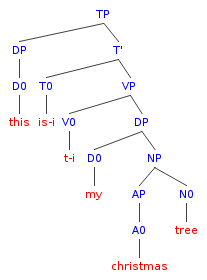
\includegraphics[scale=.6]{material/09xmastree}
	\caption{Frohe Weihnachten!}
\end{figure}

\end{frame}

